\documentclass[journal, a4paper]{IEEEtran}

% some very useful LaTeX packages include:

%\usepackage{cite}      % Written by Donald Arseneau
                        % V1.6 and later of IEEEtran pre-defines the format
                        % of the cite.sty package \cite{} output to follow
                        % that of IEEE. Loading the cite package will
                        % result in citation numbers being automatically
                        % sorted and properly "ranged". i.e.,
                        % [1], [9], [2], [7], [5], [6]
                        % (without using cite.sty)
                        % will become:
                        % [1], [2], [5]--[7], [9] (using cite.sty)
                        % cite.sty's \cite will automatically add leading
                        % space, if needed. Use cite.sty's noadjust option
                        % (cite.sty V3.8 and later) if you want to turn this
                        % off. cite.sty is already installed on most LaTeX
                        % systems. The latest version can be obtained at:
                        % http://www.ctan.org/tex-archive/macros/latex/contrib/supported/cite/

\usepackage{graphicx}   % Written by David Carlisle and Sebastian Rahtz
                        % Required if you want graphics, photos, etc.
                        % graphicx.sty is already installed on most LaTeX
                        % systems. The latest version and documentation can
                        % be obtained at:
                        % http://www.ctan.org/tex-archive/macros/latex/required/graphics/
                        % Another good source of documentation is "Using
                        % Imported Graphics in LaTeX2e" by Keith Reckdahl
                        % which can be found as esplatex.ps and epslatex.pdf
                        % at: http://www.ctan.org/tex-archive/info/

%\usepackage{psfrag}    % Written by Craig Barratt, Michael C. Grant,
                        % and David Carlisle
                        % This package allows you to substitute LaTeX
                        % commands for text in imported EPS graphic files.
                        % In this way, LaTeX symbols can be placed into
                        % graphics that have been generated by other
                        % applications. You must use latex->dvips->ps2pdf
                        % workflow (not direct pdf output from pdflatex) if
                        % you wish to use this capability because it works
                        % via some PostScript tricks. Alternatively, the
                        % graphics could be processed as separate files via
                        % psfrag and dvips, then converted to PDF for
                        % inclusion in the main file which uses pdflatex.
                        % Docs are in "The PSfrag System" by Michael C. Grant
                        % and David Carlisle. There is also some information
                        % about using psfrag in "Using Imported Graphics in
                        % LaTeX2e" by Keith Reckdahl which documents the
                        % graphicx package (see above). The psfrag package
                        % and documentation can be obtained at:
                        % http://www.ctan.org/tex-archive/macros/latex/contrib/supported/psfrag/

%\usepackage{subfigure} % Written by Steven Douglas Cochran
                        % This package makes it easy to put subfigures
                        % in your figures. i.e., "figure 1a and 1b"
                        % Docs are in "Using Imported Graphics in LaTeX2e"
                        % by Keith Reckdahl which also documents the graphicx
                        % package (see above). subfigure.sty is already
                        % installed on most LaTeX systems. The latest version
                        % and documentation can be obtained at:
                        % http://www.ctan.org/tex-archive/macros/latex/contrib/supported/subfigure/

\usepackage{url}        % Written by Donald Arseneau
                        % Provides better support for handling and breaking
                        % URLs. url.sty is already installed on most LaTeX
                        % systems. The latest version can be obtained at:
                        % http://www.ctan.org/tex-archive/macros/latex/contrib/other/misc/
                        % Read the url.sty source comments for usage information.

%\usepackage{stfloats}  % Written by Sigitas Tolusis
                        % Gives LaTeX2e the ability to do double column
                        % floats at the bottom of the page as well as the top.
                        % (e.g., "\begin{figure*}[!b]" is not normally
                        % possible in LaTeX2e). This is an invasive package
                        % which rewrites many portions of the LaTeX2e output
                        % routines. It may not work with other packages that
                        % modify the LaTeX2e output routine and/or with other
                        % versions of LaTeX. The latest version and
                        % documentation can be obtained at:
                        % http://www.ctan.org/tex-archive/macros/latex/contrib/supported/sttools/
                        % Documentation is contained in the stfloats.sty
                        % comments as well as in the presfull.pdf file.
                        % Do not use the stfloats baselinefloat ability as
                        % IEEE does not allow \baselineskip to stretch.
                        % Authors submitting work to the IEEE should note
                        % that IEEE rarely uses double column equations and
                        % that authors should try to avoid such use.
                        % Do not be tempted to use the cuted.sty or
                        % midfloat.sty package (by the same author) as IEEE
                        % does not format its papers in such ways.

\usepackage{amsmath}    % From the American Mathematical Society
                        % A popular package that provides many helpful commands
                        % for dealing with mathematics. Note that the AMSmath
                        % package sets \interdisplaylinepenalty to 10000 thus
                        % preventing page breaks from occurring within multiline
                        % equations. Use:
%\interdisplaylinepenalty=2500
                        % after loading amsmath to restore such page breaks
                        % as IEEEtran.cls normally does. amsmath.sty is already
                        % installed on most LaTeX systems. The latest version
                        % and documentation can be obtained at:
                        % http://www.ctan.org/tex-archive/macros/latex/required/amslatex/math/



% Other popular packages for formatting tables and equations include:

%\usepackage{array}
% Frank Mittelbach's and David Carlisle's array.sty which improves the
% LaTeX2e array and tabular environments to provide better appearances and
% additional user controls. array.sty is already installed on most systems.
% The latest version and documentation can be obtained at:
% http://www.ctan.org/tex-archive/macros/latex/required/tools/

% V1.6 of IEEEtran contains the IEEEeqnarray family of commands that can
% be used to generate multiline equations as well as matrices, tables, etc.

% Also of notable interest:
% Scott Pakin's eqparbox package for creating (automatically sized) equal
% width boxes. Available:
% http://www.ctan.org/tex-archive/macros/latex/contrib/supported/eqparbox/

% *** Do not adjust lengths that control margins, column widths, etc. ***
% *** Do not use packages that alter fonts (such as pslatex).         ***
% There should be no need to do such things with IEEEtran.cls V1.6 and later.

% \usepackage[linesnumbered,boxed]{algorithm2e}

\usepackage{listings}
\usepackage{pythonhighlight}

\usepackage{multicol}

\usepackage{framed}
\usepackage[colorlinks,linkcolor=blue,citecolor=blue,anchorcolor=blue]{hyperref}

% Your document starts here!
\begin{document}
\begin{titlepage}

\newcommand{\HRule}{\rule{\linewidth}{0.5mm}} % Defines a new command for the horizontal lines, change thickness here

\center % Center everything on the page
 %----------------------------------------------------------------------------------------
%	LOGO SECTION
%----------------------------------------------------------------------------------------

~\\[1cm]
\includegraphics{SCUT.png}\\[2cm] % Include a department/university logo - this will require the graphicx package

%----------------------------------------------------------------------------------------
%	TITLE SECTION
%----------------------------------------------------------------------------------------

\HRule \\[1cm]
{ \huge \bfseries The Experiment Report of \textit{Machine Learning} }\\[0.6cm] % Title of your document
\HRule \\[2cm]
%----------------------------------------------------------------------------------------
%	HEADING SECTIONS
%----------------------------------------------------------------------------------------


\textsc{\LARGE \textbf{School:} School of Software Engineering}\\[1cm]
\textsc{\LARGE \textbf{Subject:} Software Engineering}\\[2cm] 

 
%----------------------------------------------------------------------------------------
%	AUTHOR SECTION
%----------------------------------------------------------------------------------------

\begin{minipage}{0.4\textwidth}
\begin{flushleft} \large
\emph{Author:}\\
Lvjia Chen % Your name
\end{flushleft}
\end{minipage}
~
\begin{minipage}{0.4\textwidth}
\begin{flushright} \large
\emph{Supervisor:} \\
Mingkui Tan % Supervisor's Name
\end{flushright}
\end{minipage}\\[2cm]
~
\begin{minipage}{0.4\textwidth}
\begin{flushleft} \large
\emph{Student ID:}\\
201630664062
\end{flushleft}
\end{minipage}
~
\begin{minipage}{0.4\textwidth}
\begin{flushright} \large
\emph{Grade:} \\
Undergraduate
\end{flushright}
\end{minipage}\\[2cm]

% If you don't want a supervisor, uncomment the two lines below and remove the section above
%\Large \emph{Author:}\\
%John \textsc{Smith}\\[3cm] % Your name

%----------------------------------------------------------------------------------------
%	DATE SECTION
%----------------------------------------------------------------------------------------

{\large \today}\\[2cm] % Date, change the \today to a set date if you want to be precise

 
%----------------------------------------------------------------------------------------

\vfill % Fill the rest of the page with whitespace

\end{titlepage}

% Define document title and author
	\title{Face Detection Based on AdaBoost Algorithm}
	\maketitle

% Write abstract here
\begin{abstract}
\begin{bfseries}
AdaBoost is one of the most classic Boosting methods. In this report, we will try to solve a face classification problem based on a small dataset using AdaBoost. A few theory and methodology of AdaBoost will be exhibited, followed by several experiments.  
\end{bfseries}
\end{abstract}

% Each section begins with a \section{title} command
\section{Introduction}
	% \PARstart{}{} creates a tall first letter for this first paragraph
\PARstart{B}{oosting} is a machine learning ensemble meta-algorithm for primarily reducing bias, and also variance in supervised learning, and a family of machine learning algorithms that convert weak learners to strong ones.[\ref{href:Boosting}]

AdaBoost, short for Adaptive Boosting, is a Boosting method using exponential loss function which emphasizes samples classified incorrectly in the previous training epoches. 

In this report, we will first explain the methodology of AdaBoost.
Equipped with the powerful tool of AdaBoost, we will solve a face classification problem and then perform face detection with cv2 APIs supporting.  

Motivations of Experiment are listed below:
    \begin{enumerate}
      \item Understand AdaBoost further
      \item Get familiar with the basic method of face detection
      \item Learn to use AdaBoost to solve the face detection problem, and combine the theory with the actual project
      \item Experience the complete process of machine learning   
    \end{enumerate}

% Main Part
\section{Methods and Theory}
Here we will briefly introduce some important facts of AdaBoost (rather than a complete whole of the mathematical derivation process or the statistical guarantee proving of AdaBoost).

From the perspective of additive model, the AdaBoost model $H\left(X_i\right)$ can be regarded as a linear composition of many base learners $h_m\left(X_i\right)$, where $\alpha_m$ is the corresponding weight of $h_m\left(X_i\right)$.

\begin{equation}
H\left(X_i\right)=\sum_{m=1}^{T}{\alpha_mh_m\left(X_i\right)}\label{eq:1}
\end{equation}


\begin{equation}
H_m\left(X_i\right)=H_{m-1}\left(X_i\right)+\alpha_mh_m\left(X_i\right)
\end{equation}

AdaBoost use the exponential loss function to evaluate and minimize the loss:

\begin{equation}
L\left(H\left(X\right)\right)=\sum_{i=1}^{N}{e^{-y_iH\left(X_i\right)}}
\end{equation}

The following derivation mainly talks about the binary classification problem where the label y is from \{-1, +1\}.
When adapted to the binary classification problems, the AdaBoost model changes from equation (\ref{eq:1}) to:

\begin{equation}
H\left(X_i\right)=sign\left(\sum_{m=1}^{T}{\alpha_mh_m\left(X_i\right)}\right)
\end{equation}

Using the Reweighting method, AdaBoost tries to increase weights of those samples misclassified in the previous training epoches while decrease weights of samples classified correctly.

Let $\varepsilon_m$ be the error rate of the base learner $h_m\left(X\right)$ at epoch $m$, then $\alpha_m$ can be evaluated by:

\begin{equation}
\alpha_m=\frac{1}{2}\ln\left(\frac{1-\varepsilon_m}{\varepsilon_m}\right)
\end{equation}

The weighting vector $\omega$ is updated using:

\begin{equation}
\omega\left(m+1,i\right)=\frac{\omega\left(m,i\right)e^{-\alpha_my_ih_m\left(X_i\right)}}{Z_{m}}
\end{equation}

where $Z_{m}$ is the regularization factor:

\begin{equation}
Z_{m}=\sum_{i=1}^{N}{\omega\left(m,i\right)e^{-\alpha_my_ih_m\left(X_i\right)}}
\end{equation}

    \subsection*{The pseudocode of AdaBoost can be summarized as: }

\begin{framed}

\noindent For m = 1, 2, ..., T: 

    train $h_m\left(X\right)$ based on the sample weight $\omega_m$

    calculate the error rate $\varepsilon_m$ of the base learner $h_m\left(X\right)$

    if $\varepsilon_m\ge0.5$ then break 

$\alpha_m=\frac{1}{2}\ln\left(\frac{1-\varepsilon_m}{\varepsilon_m}\right)$ 

$Z_{m}=\sum_{i=1}^{N}{\omega\left(m,i\right)e^{-\alpha_my_ih_m\left(X_i\right)}}$

$\omega\left(m+1,i\right)=\frac{\omega\left(m,i\right)e^{-\alpha_my_ih_m\left(X_i\right)}}{Z_{m}}$

\noindent EndFor

\noindent return $H\left(X_i\right)=\sum_{m=1}^{T}{\alpha_mh_m\left(X_i\right)}$

\end{framed}

\section{Experiments}
\subsection{Dataset}
The dataset used in this experiment are from the \href{https://github.com/wujiaju/ML2018-lab-03}{example repository}. It provides 1000 pictures, of which 500 are human face RGB images and the other 500 are non-face RGB images. 

\subsection{Implementation}
\subsection*{B1 Training procedure of the AdaBoost Model}
    \begin{enumerate}
\item Initialize training set weights $\omega$, each training sample is given the same weight $\frac{1}{N}$. 
\item Training a base classifier(Here we use a decision tree, DecisionTreeClassifier, from sklearn.tree library) based on the current sample weights. 
\item Calculate the classification error rate $\varepsilon$ of the base classifier on the training set. 
\item Calculate the parameter $\alpha$ according to the classification error rate $\varepsilon$. 
\item Update training set weights $\omega$. 
\item Repeat steps 2-5 above for iteration. The number of iterations is based on the number of classifiers. 
    \end{enumerate}

\subsection*{B2. Face Classification}
      \begin{enumerate}
\item Load data set data. The images are converted into grayscale images with size of 24 * 24. Face images are labelled +1 while non-face images are labelled -1.
\item Processing image samples to extract NPD features.
\item The data set is divided into training set and validation set. In this experiment samples of the validation set takes up 25\% of the original data set. 
\item Predict and verify the accuracy on the validation set using the method in AdaBoostClassifier and use classification\_report() of the sklearn.metrics library function writes predicted result to classifier\_report.txt. \label{step:face_clf_4}
      \end{enumerate}

      \subsection*{B3. Face Detection}
Run the face\_detection.py file. Experience the OpenCV's built-in method of face detection using Haar Feature-based Cascade Classifiers. The result will be save as face\_detect\_result.jpg.

\subsection{Experiment Results}

\subsection*{C1. Result of Face Classification}
The result of face classification are written into the file report.txt according to [B2 step \ref{step:face_clf_4}]
The following report is generated by training a small dataset with 750 samples.

From the report we can see that the AdaBoost model gets lower loss estimate than a single weaker classifier. This shows that by using the AdaBoost method, we can combine weak classifiers to get a better classified performance.

\subsection*{*C2. Loss Estimate During AdaBoost Training}
This subsection is not required in the experiment specification. It is just a small loss etimate test performed by myself. %(注:这个小节的内容并不是实验要求,只是我自己做的一个损失函数评估的小实验)

The following graphs depict the 0/1 loss(fig \ref{fig:losses_01}) and exponential loss(fig \ref{fig:losses_exp}) both decrease as more and more weaker classifiers are aggregated. After epoch 6, the training loss decreases while the val loss increases, which shows the model is likely to become overfitting.

\begin{figure}[!hbt]
        \begin{center}
        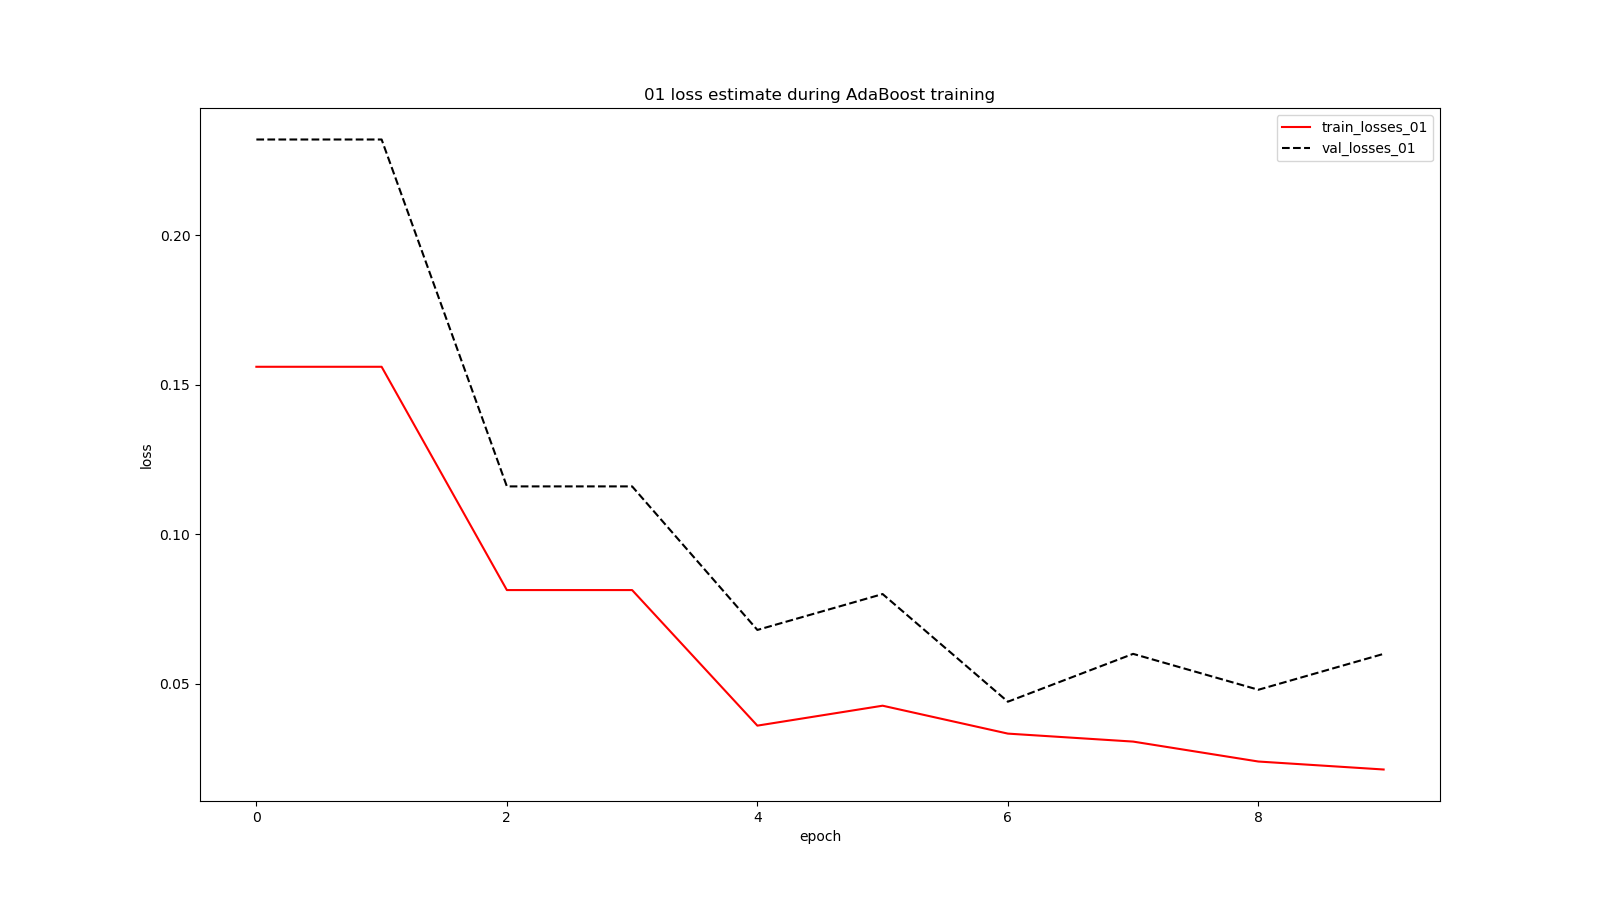
\includegraphics[width=\columnwidth]{AdaBoost_losses_01}
        \caption{Zero/One Losses during AdaBoost Training.}
        \label{fig:losses_01}
        \end{center}
\end{figure}

\begin{figure}[!hbt]
        \begin{center}
        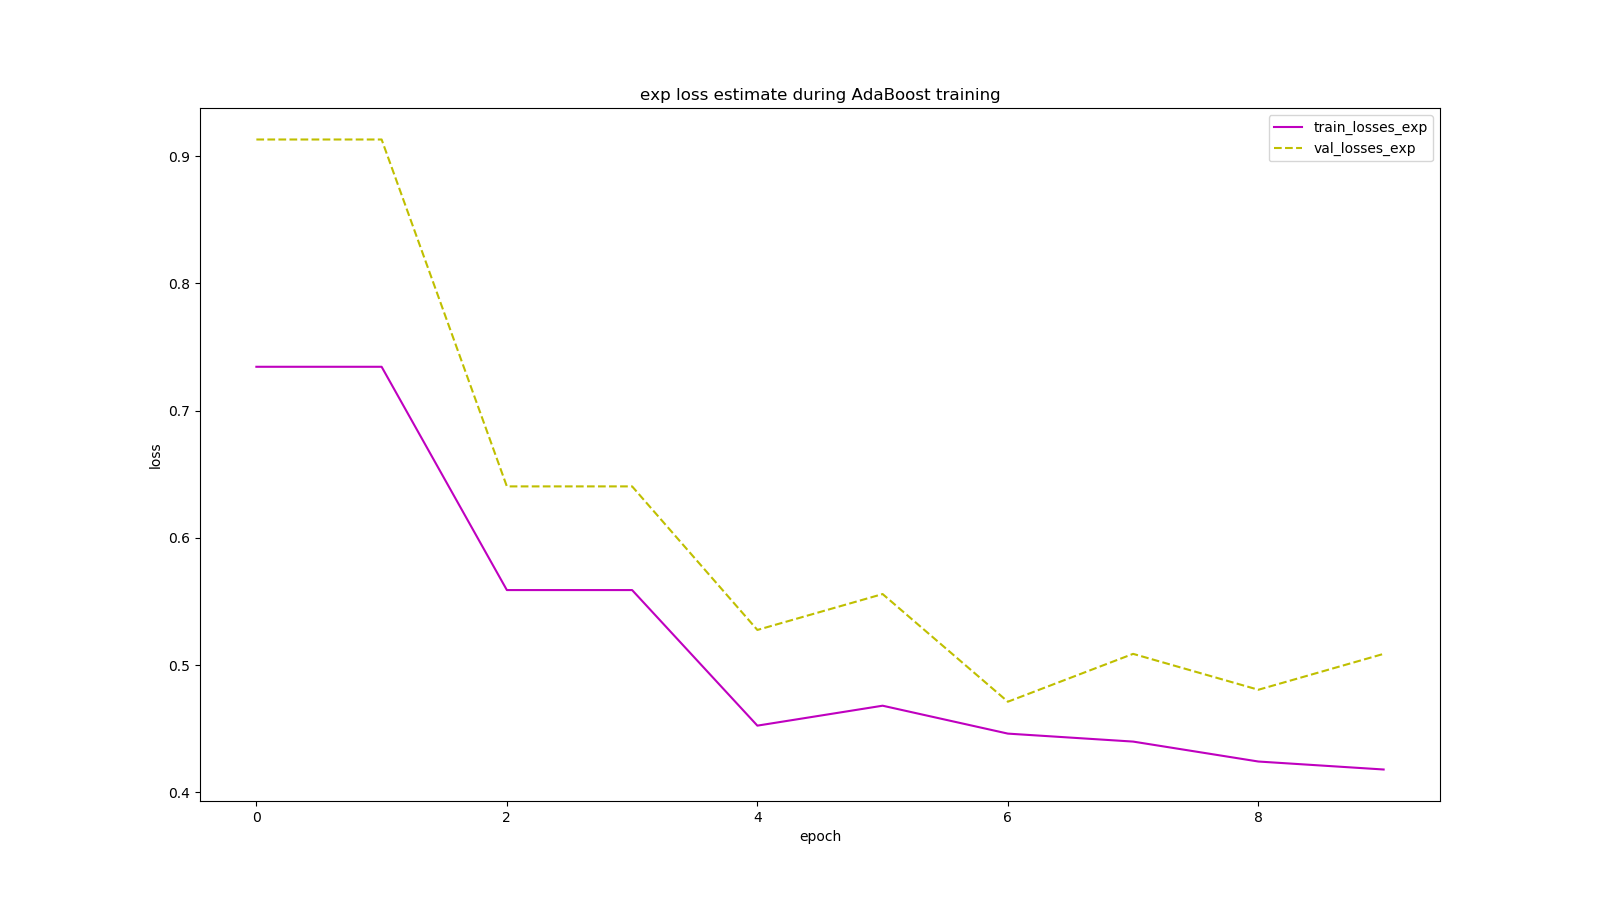
\includegraphics[width=\columnwidth]{AdaBoost_losses_exp}
        \caption{Exponential Losses during AdaBoost Training.}
        \label{fig:losses_exp}
        \end{center}
\end{figure}

\section{Conclusion}
In this report, we learn about the methodology about AdaBoost. Then we perform a face classification problem using AdaBoost. This report further estimates loss of the dataset during AdaBoost training process.

\section{References}
\begin{enumerate}
\item \href{https://www.zybuluo.com/liushiya/note/1305570}{Face Detection Based on AdaBoost Algorithm}
\item Prof.Mingkui Tan. ''Ensemble.ppt''
\item Prof. Mingkui Tan. ''Boosting Method(AdaBoost, GBDT and XGBoost).pdf''
\item Zhihua zhou. Machine Learning
\item Hang Li. Statistical Learning Method
\item \href{https://en.wikipedia.org/wiki/AdaBoost}{Wikipedia. AdaBoost}
\item \href{https://en.wikipedia.org/wiki/Boosting_(machine_learning)}{Wikipedia. Boosting} \label{href:Boosting}
\end{enumerate}

\newpage

\begin{mulitcols}{2}
\subsection{report.txt}
\begin{lstlisting}
1.loss estimate of a single weak classifier 
(a sklearn.tree.DecisionTreeClassifier with max_depth = 1):
timestamp: 2018-11-17 10:51:47.031201

  train_loss_exp = 0.750212
  train_loss_01  = 0.162667
  val_loss_exp   = 0.884968
  val_loss_01    = 0.220000

  classification_report of train data:
                precision    recall  f1-score   support

          face       0.88      0.78      0.82       370
      non-face       0.80      0.90      0.85       380

     micro avg       0.84      0.84      0.84       750
     macro avg       0.84      0.84      0.84       750
  weighted avg       0.84      0.84      0.84       750


  classification_report of val data:
                precision    recall  f1-score   support

          face       0.88      0.67      0.76       130
      non-face       0.72      0.90      0.80       120

     micro avg       0.78      0.78      0.78       250
     macro avg       0.80      0.78      0.78       250
  weighted avg       0.80      0.78      0.78       250
    
2.loss estimate of AdaBoost 
(base classifier: sklearn.tree.DecisionTreeClassifier with max_depth = 1):
timestamp: 2018-11-17 10:55:24.688709
    
  train_loss_exp = 0.418021
  train_loss_01  = 0.021333
  val_loss_exp   = 0.508904
  val_loss_01    = 0.060000

  classification_report of train data:
                precision    recall  f1-score   support

          face       0.98      0.97      0.98       370
      non-face       0.97      0.98      0.98       380

     micro avg       0.98      0.98      0.98       750
     macro avg       0.98      0.98      0.98       750
  weighted avg       0.98      0.98      0.98       750


  classification_report of val data:
                precision    recall  f1-score   support

          face       0.98      0.91      0.94       130
      non-face       0.91      0.97      0.94       120

     micro avg       0.94      0.94      0.94       250
     macro avg       0.94      0.94      0.94       250
  weighted avg       0.94      0.94      0.94       250

\end{lstlisting}
\end{mulitcols}

\newpage

\section{Appendix}

\subsection{report.txt}
\begin{lstlisting}
1.loss estimate of a single weak classifier 
(a sklearn.tree.DecisionTreeClassifier with max_depth = 1):
timestamp: 2018-11-17 10:51:47.031201

  train_loss_exp = 0.750212
  train_loss_01  = 0.162667
  val_loss_exp   = 0.884968
  val_loss_01    = 0.220000

  classification_report of train data:
                precision    recall  f1-score   support

          face       0.88      0.78      0.82       370
      non-face       0.80      0.90      0.85       380

     micro avg       0.84      0.84      0.84       750
     macro avg       0.84      0.84      0.84       750
  weighted avg       0.84      0.84      0.84       750


  classification_report of val data:
                precision    recall  f1-score   support

          face       0.88      0.67      0.76       130
      non-face       0.72      0.90      0.80       120

     micro avg       0.78      0.78      0.78       250
     macro avg       0.80      0.78      0.78       250
  weighted avg       0.80      0.78      0.78       250
    
2.loss estimate of AdaBoost 
(base classifier: sklearn.tree.DecisionTreeClassifier with max_depth = 1):
timestamp: 2018-11-17 10:55:24.688709
    
  train_loss_exp = 0.418021
  train_loss_01  = 0.021333
  val_loss_exp   = 0.508904
  val_loss_01    = 0.060000

  classification_report of train data:
                precision    recall  f1-score   support

          face       0.98      0.97      0.98       370
      non-face       0.97      0.98      0.98       380

     micro avg       0.98      0.98      0.98       750
     macro avg       0.98      0.98      0.98       750
  weighted avg       0.98      0.98      0.98       750


  classification_report of val data:
                precision    recall  f1-score   support

          face       0.98      0.91      0.94       130
      non-face       0.91      0.97      0.94       120

     micro avg       0.94      0.94      0.94       250
     macro avg       0.94      0.94      0.94       250
  weighted avg       0.94      0.94      0.94       250

\end{lstlisting}

\subsection{Core Code of AdaBoost Training (written in python)}

\begin{python} 
import math
import copy
import numpy as np

class AdaBoostClassifier:
    '''A simple AdaBoost Classifier.
    Only support binary classification in which 
    the label y is from {-1, +1} currently.
    '''

    def __init__(self, weak_classifier, n_weakers_limit):
        '''Initialize AdaBoostClassifier

        Args:
            weak_classifier: A instance of weak classifier, 
            which is recommend to be 
            sklearn.tree.DecisionTreeClassifier.
            n_weakers_limit: The maximum number of weak classifier 
            the model can use.
        '''
        self.weak_clf = weak_classifier
        self.n_weakers_limit = n_weakers_limit

    def is_good_enough(self):
        '''Optional'''
        pass

    def fit(self,X,y):
        '''Build a boosted classifier from the training set (X, y).
        Args:
            X: An ndarray indicating the samples to be trained, 
            which shape should be (n_samples,n_features).
            y: An ndarray indicating the ground-truth labels 
            correspond to X, which shape should be (n_samples,1),
               where the class label y[i, 0] is from {-1, +1}.
        '''
        w = np.ones(y.shape)
        w = w / w.sum() # regularization

        self.a = []
        self.base_clfs = []

        for i in range(self.n_weakers_limit):
            base_clf = copy.copy(self.weak_clf)
            base_clf.fit(X, y.flatten(), w.flatten())

            y_pred = base_clf.predict(X).reshape((-1, 1))

            err_rate = w.T.dot(y_pred != y)[0][0] / w.sum()

            if err_rate > 1 / 2 or err_rate == 0.0:
                break

            weight_param_a = math.log((1 - err_rate) / err_rate) / 2

            self.base_clfs.append(base_clf)
            self.a.append(weight_param_a)

            w = w * np.exp(-weight_param_a * y * y_pred)
            w = w / w.sum() # regularization

            # prevent overfiting
            # if self.is_good_enough():
            #     break;

    def predict_scores(self, X):
        pass

    def predict(self, X, threshold=0):
        pass

\end{python}

% Your document ends here!
\end{document}